\Question{Variational Inference}


In many Deep Learning labs, researchers are now focusing on Variational Inference approaches for Bayesian neural networks, where the weights are distributions instead of point estimates and thus the ouput is a very complicated distribution. In summary, variational inference is a technique that approximates intractable integrals that appear in Bayesian inference. Like generative models such as LDA and QDA, Variational Inference is especially effective in approximating the true distribution $ P(X) $, where $ X $ is the distribution of the data set. Variational Inference is also effective in approximating models that are, in a probablistic persepctive, based on MAP or MLE, like neural networks. We will focus on both aspects in the problem.

In essence, like Expectation-Maximization, Variational Inference reduces $ X $ into a set of latent/unknown variables $ Z = \left\{ Z_1, Z_2, ..., Z_n \right\}$ and attempts to approximate $ P(Z|X) $, which is an intractable distribution to calculate, with a simpler distribution $ Q(Z|X) $.


\begin{Parts}

\Part
We will now begin with KL divergence. As a warmup, given two distributions $ p = N(\mu_1, \sigma_2)$ and $ q = N(\mu_2, \sigma_2) $, find $ D_{KL}(p||q) $ in terms of $ \mu_1, \sigma_2, \mu_2, \sigma_2 $.

\begin{solution}

Let $ p(x) = N(\mu_1, \sigma_1) $ and $ q(x) = N(\mu_1, \sigma_2)$. \[ D_{KL}(p(x), q(x)) = - \int p(x)\log\frac{q(x)}{p(x)}dx = - \int p(x) \log q(x) dx + \int p(x) \log p(x) dx \] After plugging in the normal/multivariate equation for normal distribution, we get that \[ \int p(x) \log p(x) dx = \frac{1}{2} (\log 2 \pi \sigma_1^2+1) \]
and \[ \int p(x) \log q(x) dx = \frac{\sigma_1^2 + (\mu_1 - \mu_2)^2}{2 \sigma_2^2} + \frac{1}{2} \log (2 \pi \sigma_2^2) \].
Therefore, \[ D_{KL}(p(x), q(x)) =  \frac{\sigma_1^2 + (\mu_1 - \mu_2)^2}{2 \sigma_2^2} + \log \frac{\sigma_2}{\sigma_1} \]

\end{solution}


\Part
As mentioned in the description of the problem, the ultimate goal is to calculate the posterior distribution $ P(Z|X) $. Remember in MAP that we have: \[  P(Z|X) = \frac{P(X|Z)P(Z)}{P(X)} = \frac{P(X|Z)P(Z)}{\int_{Z} P(X,Z) \,dZ}  \]
In homework, we learned that to maximize $ P(Z|X) $, the denominator can be ignored, as it is intractable. However, MAP is not enough, as it calculates a point estimate that maximizes $ P(Z|X) $, which is not a distribution!
As the number of data points $ X $ goes to infinite, $ P(Z|X) $ will become infinitely more complicated and harder to compute the exact distribution. Therefore, we approximate $ P(Z|X) $ with $ Q(Z|X)$. \\\\ In order to find $ Q(Z|X) $, we want to minimize the KL divergence $ D_{KL}[Q(Z|X)||P(Z|X)] $. Prove that this divergence reduces to:

\[ \log P(X) -D_{KL}[Q(Z|X)||P(Z|X)] = E_{z\sim Q}[\log P(X|z)] - D_{KL}[Q(Z|X)||P(Z)] \]
\\Hint: Directly expand the equation and apply Bayes Rule for $ P(Z|X) $ with $ P(Z) $ as our prior on $ Z $.

\begin{solution}

\[  D_{KL}[Q(Z|X)||P(Z|X)] = - \int Q(Z|X)\frac{Q(Z|X)}{P(Z|X)}dz = E_{z\sim Q}[\log Q(z|X)-\log P(z|X)] \]
We then plug in $ P(z|X) = \frac{P(X|z)P(z)}{P(x)}$ from Bayes Rule:
\[  D_{KL}[Q(Z|X)||P(Z|X)] = E_{z\sim Q}[\log Q(z|X) - \log P(X|z) - \log P(z)] + \log P(X)  \] We can take  $ E_{z\sim Q}[\log Q(z|X)] $ and   $ E_{z\sim Q}[\log P(z)] $ out of the equation by substituting,   \[ D[Q(Z|X)||Q(Z)] =E_{z\sim Q}[\log Q(z|X)-\log P(z)] \]
Finally, our substitutions yield the ELBO equation!
\[  D_{KL}[Q(Z|X)||P(Z|X)] = -E_{z\sim Q}[\log P(X|z)] + D[Q(Z|X)||Q(Z)] + \log P(X)  \]
\[ \log P(X) -D_{KL}[Q(Z|X)||P(Z|X)] = E_{z\sim Q}[\log P(X|z)] - D_{KL}[Q(Z|X)||P(Z)] \]


\end{solution}


\Part
The equation above is called the ELBO equation, which means Evidence Lower Bound. This is what we are trying to maximize in Variational Inference We will now analyze the equation above. Which side of the equation is intractable? Which side is tractable? Why is this equation called evidence lower bound? (Hint: In generative models, we are trying to maximize $ P(X) $)

\begin{solution}

The left hand side of ELBO is intractable. $ P(X) $, or the probability distribution of data is oftentimes a very complicated distribution. Furthermore, since $ P(Z|X) $ is intractable, $ D_{KL}[Q(Z|X)||P(Z|X)] $ is also hard to compute.\\\\On the right side, we have two terms, $ E_{z\sim Q}[\log P(X|z)] $ and $ D_{KL}[Q(Z|X)||P(Z)] $. Since we know $ Q(Z|X) $, which is our approximate distribution and usually approximated as a multivariate gaussian, $ E_{z\sim Q}[\log P(X|z)] $ is feasible.  $ D_{KL}[Q(Z|X)||P(Z)] $ is tractable since $ P(Z) $ symbolizes our prior, in which we typically define it as $ N(0, I) $.\\\\Since both sides of the equation are tractable and intractable respectively, we can use the tractable side of ELBO to estimate the intractable side. Remember that we are trying to maximize $ P(X) $; however, we subtract $ D_{KL}[Q(Z|X)||P(Z|X) $ in ELBO. Because obtaining $ P(X) $ is infeasible, we can only, at best, approximate the lower bound of $ P(X) $. This is why we call this equation Evidence Lower Bound.


\end{solution}

\Part
Let's now touch upon an application of Variational Autoencoders. In essence, our latent variables $ Z $ symbolize $ N(\mu, \Sigma)$. As shown in the diagram below, we have two neural networks, the encoder and the decoder. The encoder takes in $ X $ and outputs latent variables $ Z $. Then, we sample from $ Z $ and plug it in through the second neural network to obtain our generated image $ X' $. $ ||X - X'||^2 $ and $ KL[N(\mu(X), \Sigma(X))|| N(0, I)] $ represent the respective loss functions.\\\\To train both networks, we backpropagate from our generated $ X' $ all the way back to input $ X $. However, backpropagation cannot go through random nodes, which is our sampling of $ z $.\\\\There is, in fact, a simple solution that allows us backpropagate all the way back to $ X $. Using the fact that we can represent our sampling of $ z $ as $ \mu(X) + e*\Sigma(X) $, where $ e $ is $ N(0, 1) $, redraw the nodes such that the neural network can backpropagate.
\begin{center}
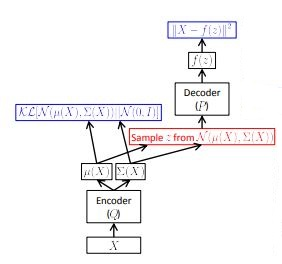
\includegraphics[width=3in]{src/problems/variational_inference/VI1.jpg}
\end{center}

\begin{solution}

\begin{center}
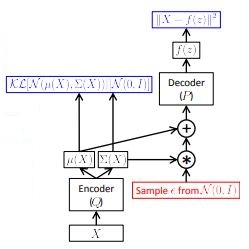
\includegraphics[width=3in]{src/problems/variational_inference/VI2.jpg}
\end{center}
By isolating the "randomization", we can backpropagate through the exact values of $ \mu(X) $, and $ \Sigma(X) $ and chop off the gradient values at the $ e $ node.

\end{solution}

\end{Parts}
